\subsection{Session page}
To create a session the user must first reach the Sessions component, which can be accessed by clicking on the “Sessions” button on the navbar. The session page will have the URL /admin/sessions. A session cannot be created until both a course and a question are present in the database. Therefore, the user will have to visit both the dashboard and the question page, before accessing the session page. In the figure \ref{fig:sessionPage} shows the session page, in this figure a session has already been created called “Test Økt”. Since this session is created and includes some questions, the Session component is visible on the Sessions component to the right side of the page. If there are no sessions for the chosen course, then only the Sessions component will be displayed on the page. Although if this is the case, then the Sessions component will not have any sessions in the list.
The Session component contains a search bar and a select box identical to the ones in the question page. The component also contains a list that will include all the current sessions created for the chosen subject. Just like in the list on the question page, the list on the session page will send a socket emit message to the server in order to keep its session list up to date. The list will be updated whenever the Session component is loaded, a new session is created or whenever the chosen course is changed. Once the Session component is visible, the information displayed on the component will vary depending on the current question being selected. You can easily change between the available session and its questions by clicking on their name. On figure \ref{fig:sessionPage} you can see that the session “Test Økt” has opened the question “Text Question”. 
The information displayed on the Session component comes from a component by the name DisplayQuestion. The DisplayQuestion is a component that is used whenever an admin is going to watch question information in the same style as in an active session. Essentially the component is used on the session page and on the user profile page. The DisplayQuestion component uses a vue card, which makes it easier to toggle between showing the question information and the solution.  The DisplayQuestion contains unique components for solution and answer for each question type. %TO BE CONTINUED…
\begin{figure}[H]
	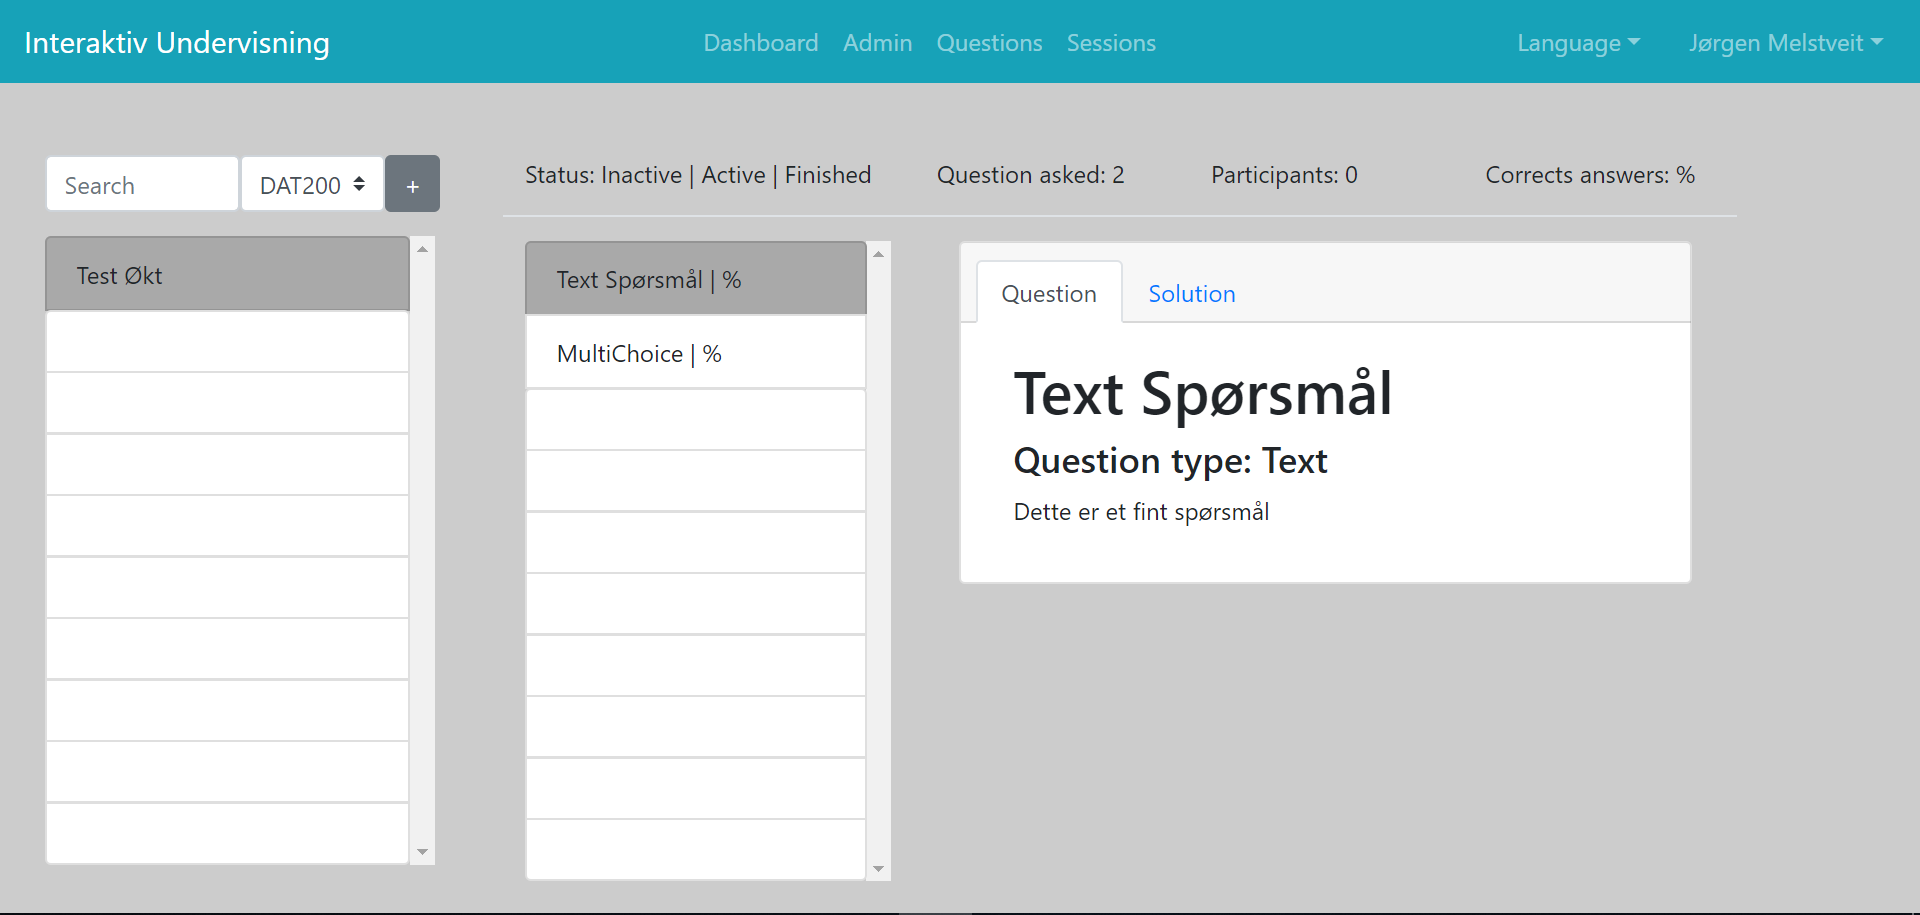
\includegraphics[width=0.80\linewidth]{sessionPage}
	\caption{This figure display the session page.}
	\label{fig:sessionPage}
\end{figure}